\chapter{Spectral Neural Representation of Seamless Textures}

Textures play a fundamental role in computer graphics, enabling the creation of visually appealing and realistic virtual environments. They provide essential information about the materials, surfaces, and spatial variations present in the virtual scene, enriching the visual experience with intricate details, patterns, and micro-scale level characteristics that would be very difficult to model otherwise.

Within this scope, \textit{periodic textures} stand out as an important example that models repeating patterns with regularity along one or more dimensions. Periodic textures are specially useful to represent materials found in domains such as architecture, textiles, and industrial design. Capturing the essence of such textures is an important task to bridge the gap between virtual scenes and their real-world counterparts.


Traditionally, texture tiles are depicted as discrete digital images. We propose to use our multiresolution INR to represent seamless periodic textures in a continuous, compact and fast to evaluate representation. In this chapter we extend deep sinusoidal neural networks to \textit{periodic neural networks}. We prove that if we initialize the first layer of a sinusoidal INR with frequencies that are integer multiples of a period $P$, then the entire INR will be periodic with period $P$.  This is due to the fact that the composition of sinusoidal layers expands as a sum of sines with frequencies given by integer combinations of the input layer, and the result is similarly periodic~\citep{novello2022understanding, yuce2022structured}. We leverage this property to fit periodic signals such as image and texture representations.


Periodic networks allows us to represent a periodic texture in a infinite domain by training it only in a small tile. When the data is non-tileable, we introduce a regularization term based on the \textit{Poisson equation} to enforce that the image produced by a periodic INR forms a seamless, tileable texture -- meaning it should tile across the plane without displaying noticeable seams or discontinuities at the tile boundary. The key idea is to enforce the INR gradient of the network to match the original gradient within the domain (Poisson equation) and to ask the INR to be equal to an image average on the domain border (periodic boundary values)~\cite{perez2003}. It is important to note that for this problem to be well-posed, the boundary must be closed. However, since our network is periodic, we are solving the Poisson problem on the torus which allows us to also require gradient matching on the domain boundary (see the results in Section \ref{s:poisson-regularization}).

% Training a sinusoidal INR to fit a given texture sample has the drawback of its image possibly being non-tileable. To avoid this, we introduce a condition for an INR to be \textit{periodic} and propose a regularization term based on the \textit{Poisson equation}. 

% The next step in our method involves defining a regularization term to \myhl{ensure that the image produced by a periodic INR forms a seamless, tileable texture -- meaning it should tile across the plane without displaying noticeable seams or discontinuities at the tile boundary}.
% To achieve this, we employ the Poisson equation which enforces the INR gradient matches the original gradient within the domain (Poisson equation) and asks the INR to be equal to an image average on the domain border (periodic boundary values)~\cite{perez2023poisson}.


Besides the periodic representation, our method leads to better representation quality of images with fewer parameters in the architecture. Additionally, based on Fourier series, we design a frequency initialization that greatly decreases the amount of possible choices for frequencies. Our experiments demonstrate that this representation is suitable for representing periodic textures, and making them seamless, and can be easily integrated to the graphics pipeline for texture mapping.


%%%%%%%%%%%%%%%%%%%%%%%%%%%%%%%%%%%%%%%%%%%%%%%%%%%%%%%%%%%%%%%%%%%%%%%%%%%%%%%%%%%%%%%
\section{Background and related methods}

The scope of this chapter is to represent seamless material textures using \textit{implicit neural representations} (INRs). Thus, it aims to encode the material texture of a surface through a periodic neural network $f_\theta:\mathbb{R}^2\to \mathcal{C}$, where $\mathcal{C}$ is a color space such as grayscale or \texttt{RGB}, and $\theta$ is the set of parameters of the netowrk. that can be trained based on data samples. More generally, this representation could be extended to the other channels of a material definition such as the specular or normal channels.

In this sense, the context is texture creation methods (procedural-based, capture-based, AI-based, and manual) with the purpose of being applied to a 3D surface by a rendering system.

Generating high-quality textured materials is challenging as they need to be visually realistic, seamlessly tileable, and have a small impact on the memory consumption of the application. For this reason, these materials are often created manually by skilled artists. In this chapter, we show that INRs can be used in those tasks.

Additionally, it is desirable to have an agnostic material representation based on industry standards that is compatible with most rendering systems. One case is the Substance 3D Sampler from~\citet{substance_sampler}, a creation platform of material collections that includes many tools for that very purpose. Next, we discuss the most relevant works that are related to our method.


\subsection{Texture representations}

Texture is ubiquitous in computer graphics. It is the key to represent visual information for the synthesis of naturalistic textures and images from photographic exemplars. Texture synthesis has grown into a mature field encompassing a variety of methods, such as: classic texture mapping \cite{blinn76}, procedural textures \cite{perlin-1985}, synthesis-by-example \cite{efros99}, and user-guided texture generation \cite{haeberli90}. \citet{pauly-2009} gives an overview of example-based texture synthesis methods. Also, \citet{etal-2010} provides an in-depth account of noise primitives for procedural texturing.
%
Recently, \citet{rethinkngtex} discusses alternative texture-mapping methods.

Most of the these previous methods target general texture patterns. However, there is a trend that investigates models of specific materials. This approach has the benefit of producing higher fidelity results by exploiting characteristics of important materials, such as wood.
\citet{dorsey-2004} studies aggregate materials that are common in nature and formed by small particles.

\subsection{Tileable Textures}

While there is a large body of research devoted to texture mapping, little work has been dedicated to synthesizing seamless tileable textures, which are important for the creation of materials. These textures have the property that when laid out in a regular grid of tiles they form a homogeneous appearance suitable for use in memory-sensitive real-time graphics.

\citet{tileinteractive} gives an overview of tile-based methods in computer graphics applications.
%
Additionally, we highlight the following methods. \citet{tilehard} presents a tile-based texture mapping algorithm that generates an arbitrarily large and non-periodic virtual texture map from the small set of stored texture tiles. \citet{Moritz2017Texture} developed an approach to synthesize tileable textures using the PatchMatch texture synthesis algorithm.
% %
These methods rely on a particular algorithm that must be incorporated into the rendering system. Our INR representation, once trained is exported to be evaluated on the graphics hardware or, alternatively, can be used to generate a material tile.

\citet{perez2003} modeled the problem of making a rectangular domain texture tileable using a Poisson solver: the boundary conditions consist of forcing the opposite sides of the domain to be equals. In the interior, they asked for the gradient of the desired texture to be equal the ground-truth gradient. This approach works only on pixel-based images. Our method allows for the definition of a regularization term that compels the training of a periodic INR to produce a seamless, tileable texture. Furthermore, we can interchange the boundary and interior equations, given that our problem is defined on the 2D torus once the network is periodic.


\subsection{Neural Textures}

Texture representations aim to integrate procedural techniques with data sample fitting. The primary trade-off lies between computational efficiency and memory usage. Promising solutions to this challenge are offered by \emph{wavelets} and \emph{neural networks}. For instance, \citet{BAJAJ-2000} tackled the memory issue by employing a wavelet-based method to encode 3D textures. Meanwhile, \citet{Gutierrez-2019} introduced a generative deep learning framework for 3D texture synthesis based on style transfer. Their results are comparable to those of patch-based approaches.



For tileable textures, \citet{deeptile} introduced an example-based texture synthesis approach using deep learning. This method creates tiles at arbitrary resolutions that closely resemble the structural components of an input texture. Similarly, \citet{zhou2022tilegen} devised a variant of StyleGAN with modifications to generate periodic material maps. While these studies utilize "data-based neural networks" and generative models, our approach employs "coordinate-based neural networks" and a spectral representational model.

In another vein, \citet{ntc2023} developed a neural compression technique tailored specifically for material textures. Meanwhile, \citet{match} presented a method based on deep neural features for graph creation, aiming at constructing procedural materials. In this context, our INR model offers a compact solution that can seamlessly integrate into a neural rendering pipeline.

\subsection{Implicit neural representations}

We have seen that Bacon \cite{bacon2021} builds upon \textit{Multiplicative filter networks} (MFNs) \cite{fathony2020multiplicative} to control frequencies in the network and represent signals at multiple scales. As this representation is analyticaly equivalent to a shallow network, it is clear that the representation can be made periodic by initializing the first layer with frequencies that are integer multiples of a period $P$. However, for deep sinusoidal MLP such as Siren or MR-Net, this may not be true, since the composition of sines can generate much more frequencies. Figure \ref{f:generated-frequencies} shows the magnitude of frequencies, computed using the Fast Fourier transform (FFT), for signals generated by the sum of sines, product of sines, product of a sine by a sum of sines, and composition of sines. It is evident that the composition of sines produces a larger number of frequencies compared to the other options.

\begin{figure}[h]
\centering
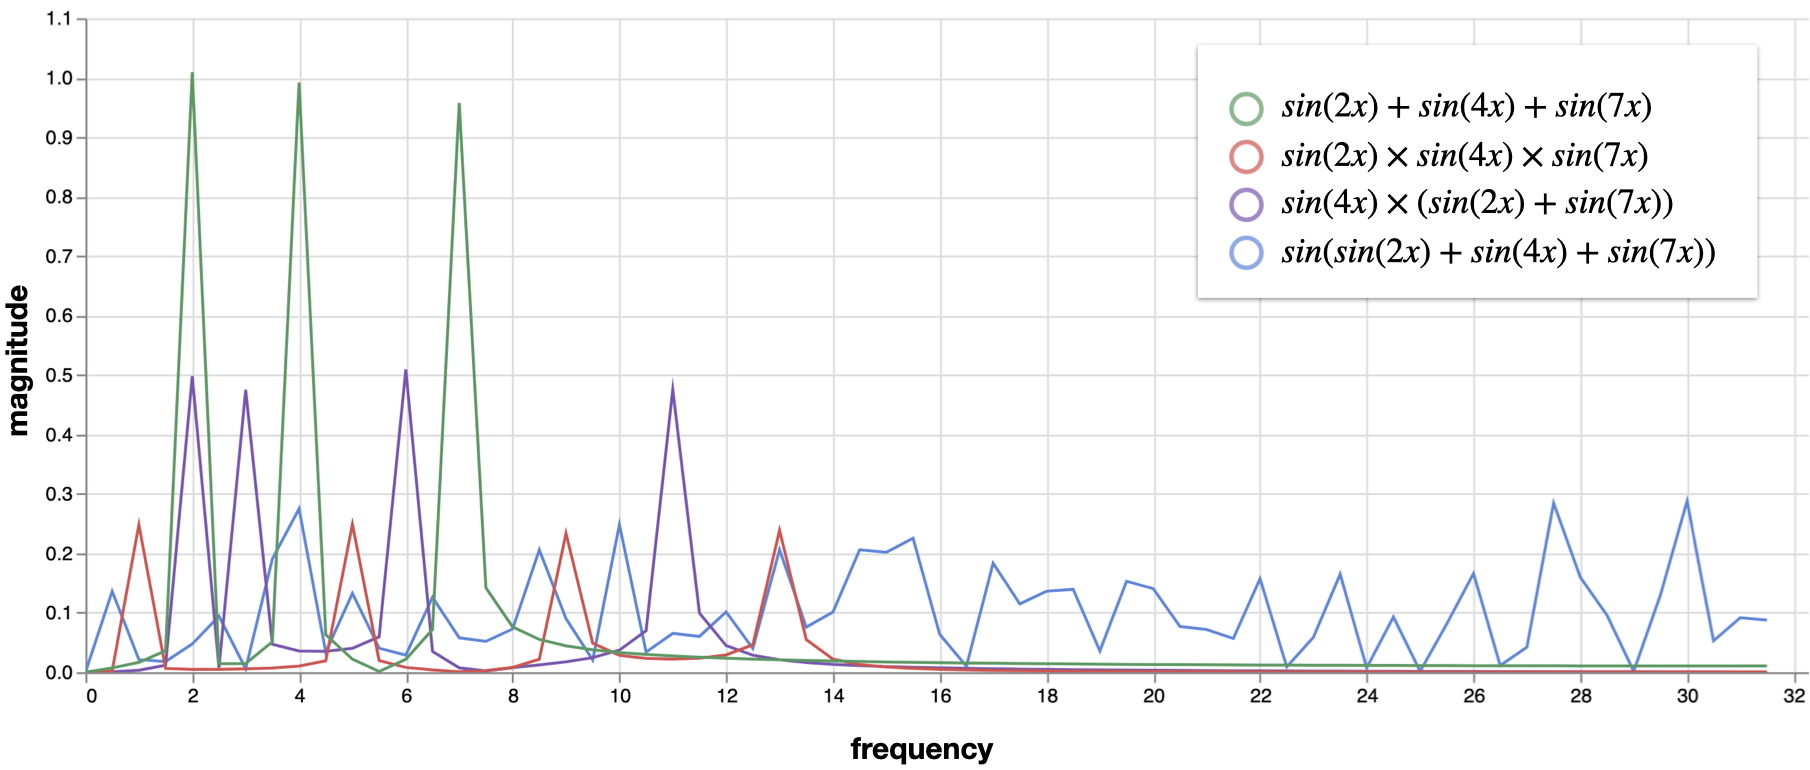
\includegraphics[width=0.80\linewidth]{img/ch6/generated_frequencies.png}
\caption{Fourier Transform of different combinations of sinusoidal functions.}
\label{f:generated-frequencies}
\end{figure}
    

Regarding seamless textures, inspired by~\cite{perez2003}, we model it as a term in the loss  function using a Poisson problem. This strategy has been explored in INRs for tasks such as compositing gradients~\cite{sitzmann2019siren} and 
%face morphing~ \cite{schardong2024neural}.
\red{problem with Schardong 2024 citation} SIREN trains the INR using only the gradients, leading to the learning of the signal up to an integral constant, which is problematic when we have multiple channels. In contrast, our training scheme incorporates both gradient and image values.


% %%%%%%%%%%%%%%%%%%%%%%%%%%%%%%%%%%%%%%%%%%%%%%%%%%%%%%%%%%%%%%%%%%%%%%%%%%%%%%%%%%%%%%%
\section{Periodic Neural Networks}

For simplicity, along this section, we assume the image's codomain to be $\mathbb{R}$, since the results can be easily extended to multiple channels.

A \textit{periodic image} $\gt{f}:\mathbb{R}^2\to \mathbb{R}$ is a function satisfying the property $\gt{f}(x) \!=\! \gt{f}(x + P)$ with $P=(P_1, P_2)\in \mathbb{R}^2$ giving the \textit{periods} along the axes $x_1$ and $x_2$.
For an example, consider the \textit{harmonic} $h(x_1, x_2)=a\sin(x_1\omega_1+x_2\omega_2+ \varphi)$ where $\omega_i\!=\!k_i\frac{2\pi}{P_i}$, with $k_i\in\Z$, are the \textit{frequencies}, $a$ is the \textit{amplitude}, and $\varphi$ is the \textit{phase shift}.
Such functions play a central role in \textit{Fourier series}, where the periodic function $\gt{f}$ can be approximated by a sum of harmonic functions.


\subsection{Shallow Sinusoidal networks}
Observe that summing harmonic functions also results in a \textit{sinusoidal network} $f:\R^2\to \R$ with a single layer:
\begin{align}\label{e-fourier_series}
    f(x) = L\circ s(x) =  c_0 + \sum_{i=1}^{n} c_i  \sin\Big(\dot{\omega_i}{ x}+ \varphi_i\Big)
\end{align}
where the \textit{first} layer $s:\R^2\to \R^{n}$ projects the input coordinates $x=(x_1,x_2)$ into a list of harmonics:
\begin{align}\label{e-firstlayer}
\displaystyle
    s(x)=\sin(\omega x +\varphi)=
    \left(
    \begin{array}{c}
        \sin\big(\dot{\omega_1}{x}+\varphi_1\big)\\
         {\footnotesize\vdots}\\
         \sin\big(\dot{\omega_{n}}{x}+\varphi_{n}\big)
    \end{array}
    \right).
\end{align}

Where $\dot{\omega_i}{x}=\omega_{i1}x_1+\omega_{i2}x_2$. Thus, the matrix $(\omega_1, \ldots, \omega_{n})$ gives the \textit{frequencies} and $(\varphi_1, \ldots, \varphi_{n})$ the \textit{phase shifts}.
The \textit{linear} layer $L$ combines the harmonics with the \textit{amplitudes} $c_i$ and adds a bias $c_0$.

For the network $f$ to be periodic with periods $(P_1,P_2)$ we can simply choose $\omega_{ij}=k_{ij}\frac{2\pi}{P_i}$, with $k_{ij}$ being integers.
Section~\ref{s-initialization} presents an initialization of $k_{ij}$ using ideas from Fourier series.

\subsection{Deep sinusoidal networks}\label{s-deep-networks}

We compose the first layer of $f$ with a hidden layer $h:\R^{n}\to \R^{m}$ to make $f$ deeper.
That is,
$f=L\circ h \circ \,s$, 
with $h\circ s(x):=\sin\big(W \cdot s(x)+b\big)$, where $W\in\R^{m\times n}$ is the \textit{hidden matrix}, and $b\in\R^{m}$ is the \textit{bias}.


\noindent The $i$th coordinate of $h$ one express as a \textit{sinusoidal perceptron}:
%
\begin{align*}
h_{i}\circ s(x)=\sin\left(\sum_{j=1}^{n} W_{ij} \sin\Big(\dot{\omega_j}{x}+\varphi_j\Big) + b_{i}\right).
\end{align*}
%
Thus, $f$ consists of multiple sine compositions. In a more general sense, a \textit{sinusoidal network} is a function constructed by combining sinusoidal perceptrons.
% %
Furthermore, by adding more hidden layers to $f$, we obtain a sinusoidal \textit{multilayer perceptron} (MLP). Training such networks can be challenging because using the sine as an activation function may lead to instability in deep architectures~\cite{taming2017}. \citet{sitzmann2019siren} overcome this by proposing SIREN, which gives a special initialization scheme for sinusoidal MLPs, providing stability during training.

Clearly, the activation function is periodic, but the network $f$ may not.
Recall that even summing periodic function may result in non-periodic function: e.g. $\sin(x)+\sin\left(\sqrt{2}x\right)$. 
Furthermore, to accurately represent a periodic function, we must have control over the network's period.

% %
In this work, we observe that by initializing the first layer $s$ of a sinusoidal MLP $f$ with integer frequencies, specifically $\omega_{ij}=k_{ij}\frac{2\pi}{P_i}$ where $k_{ij}\in\Z$, we can prove that $f$ will be periodic with period $P=(P_1,P_{2})$.
In other words, $f(x_1, x_2)=f(x_1+P_1, x_2+P_2)$.

For simplicity, let $f$ be a 1D function, i.e. $f:\R\to\R$, the general case follows analogously. 
Assuming the first layer to be periodic with period $P$, we see that its frequencies are expressed as $\omega_j=k_{j}\frac{2\pi}{P}$. 
Moreover, observe that if we prove that if each sinusoidal neuron $h(x)=\sin\left(\sum_{i=1}^n a_j\sin(\omega_j x + \varphi_i)\right)$ expands as a sum of harmonics with period $P$, then, the output of $h$ is periodic with period $P$. The proof of this fact follows from the following identity~\cite{novello2022understanding}:
\begin{align}\label{e-expansion}
    h(x)= \!\!\sum_{\textbf{l}\in\Z^n}\left[\prod_{i=1}^n J_{l_i}(a_i)\right]\sin\Big(\dot{\textbf{l}}{\omega x +\varphi}+ b\Big).
\end{align}
Since each frequency in this sum is written as $\dot{\textbf{l}}{\omega}=\frac{2\pi}{P}\dot{\textbf{l}}{\textbf{k}}$, we have that $h$ is periodic with period $P$.
We note that an expansion similar to Equation~\ref{e-expansion} was also presented in \cite{yuce2022structured}.


For sinusoidal MLP with two hidden layers, we truncate the expansion given by the expansion of the first layer. Thus the input of the second hidden layer is a finite sum of sines and Equation~\ref{e-expansion} can be applied.
For the truncation, we use the fact that the amplitudes
% $\prod_{i=1}^n J_{l_i}(a_i)$ goes rapidly to zero as $\norm{\textbf{l}}_{\infty}$ increases. This is due to the following inequality~\cite{novello2022understanding}:
% \begin{align}\label{e-upper-bound-freq}
%     \abs{\prod_{i=1}^n J_{l_i}(a_i)}<
%     \prod_{i=1}^n\frac{\left(\frac{\abs{a_i}}{2}\right)^{\norm{l_i}}}{\abs{l_i}!}.
% \end{align}
Applying induction in the above procedure implies the result:
\begin{theorem}
\label{t-periodic}
    If the first layer of a sinusoidal MLP $f$ is periodic with period $P$, then $f$ is also periodic with period $P$.
\end{theorem}

Theorem~\ref{t-periodic} allows us to use sinusoidal MLPs to represent periodic functions. 
We define a \textit{periodic INR} to be a sinusoidal MLP such that its first layer is periodic. 

\subsection{Multiresolution sinusoidal networks}\label{s-mr-networks}
\label{s-multiresolution}
To represent textures using INRs we need to represent them in multiresolution. For this, we adopt the \textit{multiresolution network} (MRnet)~\cite{paz2022,paz2023mr} as a representation. Here, a MRnet is a network $f\!:\!\R^2\!\times\! [0,N]\!\to\! \R$ defined as a sum of $N$ periodic INR $g_i:\R^2\to\R$:
\begin{align}\label{e-mrnet}
f(x,t) = c_0(t)g_0(x) + \cdots + c_{N-1}(t)g_{N-1}(x),
\end{align}
The contribution of each \textit{stage} $g_i$ in Equation~\ref{e-mrnet} is controlled by $
c_i(t)\!=\!\max\big\{0, \min\big\{1, t-i\big\}\big\}.$
This allows us to navigate in the multiresolution using a parameter $t\!=\!k+\delta$ with $k\in\mathbb{N}$ and $0\leq\delta\leq 1$:
\begin{align}\label{e-mrnet2}
f(x,t)=g_0(x)+\dots + g_k(x)+\delta g_{k+1}(x).
\end{align}

The \textit{level of details} $f(\cdot, t)$ evolve continuously.
We set the first layer of each periodic INR $g_i$ with integer frequencies, since Theorem~\ref{t-periodic} says that in this case $f$ will \textit{periodic} with respect to $x$.

\subsection{Frequency initialization}
\label{s-initialization}
The first layer of a sinusoidal INR projects the input coordinates into a list of sines (Eq.~\ref{e-firstlayer}). Next, we show that in a shallow network, this gives the frequencies of the signal represented by a Fourier series. Thus, the initialization of the first layer is important for network performance.
Following the conclusions of Theorem~\ref{t-periodic}, we define the first layer's frequencies to be integer multiples of a period.

Let $\gt{f}\!:\!\R^2\!\to\! \R$ be a periodic image (the \textit{ground-truth}) with period~$P$ and ${f}\!:\!\R^2\!\to\! \R$ be a periodic INR.
To define the integer matrix $k_{jl}$ of the first layer of $f$ we follow ideas from Fourier~series.
% . Fourier series 
If $\gt{f}\in L^1(P)$, the \textit{Fourier theorem} says that it expands in a series:
\begin{align}\label{e-fourier-expansion}
    \gt{f}(x)=\sum_{\textbf{k}\in \Z^2} c_\textbf{k} \text{e}^{i\dot{\omega_{{\textbf{k}}}}{ x}},
\end{align}
where $c_\textbf{k}$ are the \textit{Fourier coefficients}, and $\omega_{\textbf{k}}=2\pi\left(\frac{k_1}{P_1}, \frac{k_2}{P_2}\right)$ with $\textbf{k}=(k_1,k_2)$. 
%
In practice, we truncate the Fourier series summing over the integers $\textbf{k}\in[-B, B]^2$, where $B$ is a \textit{bandlimit}.
%

On the other hand, assuming $f$ to be a network with a single layer (Eq~\eqref{e-fourier_series}) and adding $\frac{\pi}{2}$ to the biases, we obtain:
\begin{align}\small
    f(x) &=  \frac{a_0}{2} + \sum_{k=1}^{n} a_k  \cos\big(\dot{\omega_k}{ x}+ \varphi_k\big)\\
    &=  c_0 + \sum_{k=1}^{n} c_k  \text{e}^{i\dot{\omega_{{k}}}{ x}}+ \sum_{k=-n}^{-1} c_k  \text{e}^{i\dot{-\omega_{\abs{k}}}{ x}},\label{e-mlp2complex}
\end{align}
where $c_k=\frac{a_{\abs{k}}}{2}\text{e}^{\text{sign}(k)i\varphi_{\abs{k}}}$ with $\varphi_0=0$, and $\omega_{j}=2\pi\left(\frac{k_{j,1}}{P_1}, \frac{k_{j,2}}{P_2}\right)$. 
%
% . Frequency initialization
Thus, for $f$ to approximate the truncated series in Eq.~\eqref{e-fourier-expansion}, we can set
the integers $k_{j}$ in a set $\textbf{K}\subset [-B,B]^n$ such that $-\textbf{K} = [-B,B]^n\setminus \textbf{K}$.

% % . Other parameters...
When $f$ contains hidden layers, we initialize its parameters following the scheme in ~\cite{sitzmann2019siren}. 
Notice that we initialized $f$ with a finite number of frequencies in the frequency set $\textbf{K}$. However, 
the layer composition produces many other frequencies as the depth of the network increases.
Equation~\ref{e-expansion} justifies this claim.


Regarding the frequency initialization of each stage $g_i$, we split the frequency set $\textbf{K}$ in $N$ subsets $\textbf{K}_i$ sorted by length.
Thus, the first layer of $g_i$ is initialized with the frequencies in $\textbf{K}_i$.
This initializes subsequent stages using only frequencies that were not chosen in previous stages enforcing the early stages to contain the lower frequencies, then as stages advance we add the higher frequencies.




\subsection{Network training}
\label{s-training}
Let $\gt{f}:\Omega\subset\R^2\to \mathcal{C}$ be an image (\textit{ground-truth}) defined in the rectangular domain $\Omega=[0,P_1]\times[0,P_2]$. 
We aim to approximate $\gt{f}$ by a periodic INR ${f}:\R^2\to \mathcal{C}$ with periods $(P_1, P_2)$ such that the resulting image is seamless. 
For this, define the weights $\omega_{ij}$ of the first layer of $f$ in the form $k_{ij}\frac{2\pi}{P_i}$ with $k_{ij}\in \Z^2$.
Again, this implies that the first layer is periodic with periods $(P_1,P_2)$, then, Theorem~\ref{t-periodic} implies that $f$ is also periodic with the same periods. 
To force the resulting texture to be seamless at the boundary $\partial \Omega$ of $\Omega$, we design a loss function based on a \textit{Poisson problem}.


Specifically, we use the Jacobian $\jac{\gt{f}}$ of $\gt{f}$ to train the periodic INR $f$.
For this, we define a matrix field $U$ such that its primitive approximates a seamless tileable texture at $\partial \Omega$.
% %
Then we enforce $\gt{f}=f$ at some region of $\Omega$. This can be modeled using:
\begin{align}\label{e-gradient-interpolant}\small
\min \int_{\Omega} \lambda\norm{{\jac{f}-U}}^2dx \text{ subject to } (1-\lambda)(\gt{f}-f)=0 \text{ in } \Omega.
\end{align}
Where $\lambda:\Omega\to [0,1]$ is a weight function indicating that $U$ should match the Jacobian of $f$ if it is close to one ($\lambda\approx 1$), and enforces $\gt{f}=f$, otherwise. 
 We propose to use this variational problem to define the following loss function to train the parameters $\theta$ of $f$.
\begin{align}\label{e-blending-no-grad}\small
\mathscr{L}(\theta)={\int_{\Omega} \lambda\norm{{\jac{f}-U}}^2dx} + {\int_{\Omega} (1-\lambda)\big(\gt{f}-f\big)^2dx}.
\end{align}
\noindent
Thus, $\mathscr{L}$ trains $f$ to \textit{seamless clone} the primitive of $U$ to $f$ in $\Omega$.
Unlike classical approaches that rely on pixel manipulation, seamless cloning operates on the image gradients.
Note that $\lambda$ depends on the position $x$. In practice, we consider it to have high values near $\partial \Omega$. As a result, the training forces the matching of the Jacobian of $f$ with $U$ near $\partial \Omega$. In fact, since $f$ is periodic, we are training it on the torus given by the identification of the opposite edges of $\Omega$.
Classical methods do not provide such flexibility.

\section{Experiments}

This section presents experiments conducted with our method for representing tileable material textures. We initiate the process by fitting a tileable pattern across various scales and evaluate its performance through qualitative and quantitative analysis.
Subsequently, we train the network using a sample that includes repetitions of the pattern, with a fundamental period smaller than the training domain. To achieve this, we employ masks to selectively exclude certain image areas during training, assessing the network's capability to reconstruct them accurately.
Furthermore, we tackle non-tileable patterns that can be rendered seamless through Poisson regularization. Finally, we offer comparative evaluations with existing methods in the field.

\subsection{Seamless Tileable Materials}\label{s-multires-2d}

We start with a single tile, matching the fundamental period of a texture, with a resolution of $1024^2$ pixels and $8$ bits per color channel in \texttt{RGB} space. We convert the  train a MRnet, using the framework in \cite{paz2023mr}, consisting of a $6$ periodic INRs (stages).
% We use periodic INRs with a single hidden layer, and heterogeneous width, as experiments indicated that we need fewer parameters to fit an image of lower resolution and low-frequency details. The initialization uses the scheme described in Sec~\ref{s-initialization}. The architecture of the hidden layer (number of input/output neurons) and the band limits of the first layer are in Table \ref{tab:mnet-architecture}.

% \pagebreak

% \begin{table}[h]
% \small
% \begin{tabular}{|l|c|l|l|}
% \hline
% \textbf{Stage} & \multicolumn{1}{l|}{\textbf{Band-Limit}} & \multicolumn{1}{l|}{\textbf{Hidden Input}} & \multicolumn{1}{l|}{\textbf{Hidden Output}} \\ \hline
%  0     & $[0, 3]\times[-3, 3]$                       & 24                                & 32                                 \\
%  1     & $[0, 6]\times[-6, 6]$                       & 48                                & 32                                 \\
%  2     & $[0, 12]\times[-12, 12]$                     & 80                                & 64                                 \\
%  3     & $[0, 24]\times[-24, 24]$                     & 192                               & 160                                \\
%  4     & $[0, 56]\times[-56, 56]$                     & 384                               & 256                                \\
%  5     & $[0, 128]\times[-128, 128]$                   & 1024                              & 512                                \\ \hline
% \end{tabular}
% \caption{M-Net architecture.}
% \end{table}\label{tab:mnet-architecture}

% \vspace{-.7cm}

% Figure \ref{f:rec_gt} presents a qualitative comparison between the original image and the reconstructed image using our method. 
% Observe that the images exhibit a high degree of similarity with a PSNR of 31.8 dB.
% Additionally, our model achieves this level of fidelity using 855,572 parameters, which is less than the number of pixels in the image (1,048,576). Our model also demonstrated the ability to encode information at multiresolution giving an even better compression compared to a traditional Mipmap.

% \begin{figure}[h]
% \centering
% 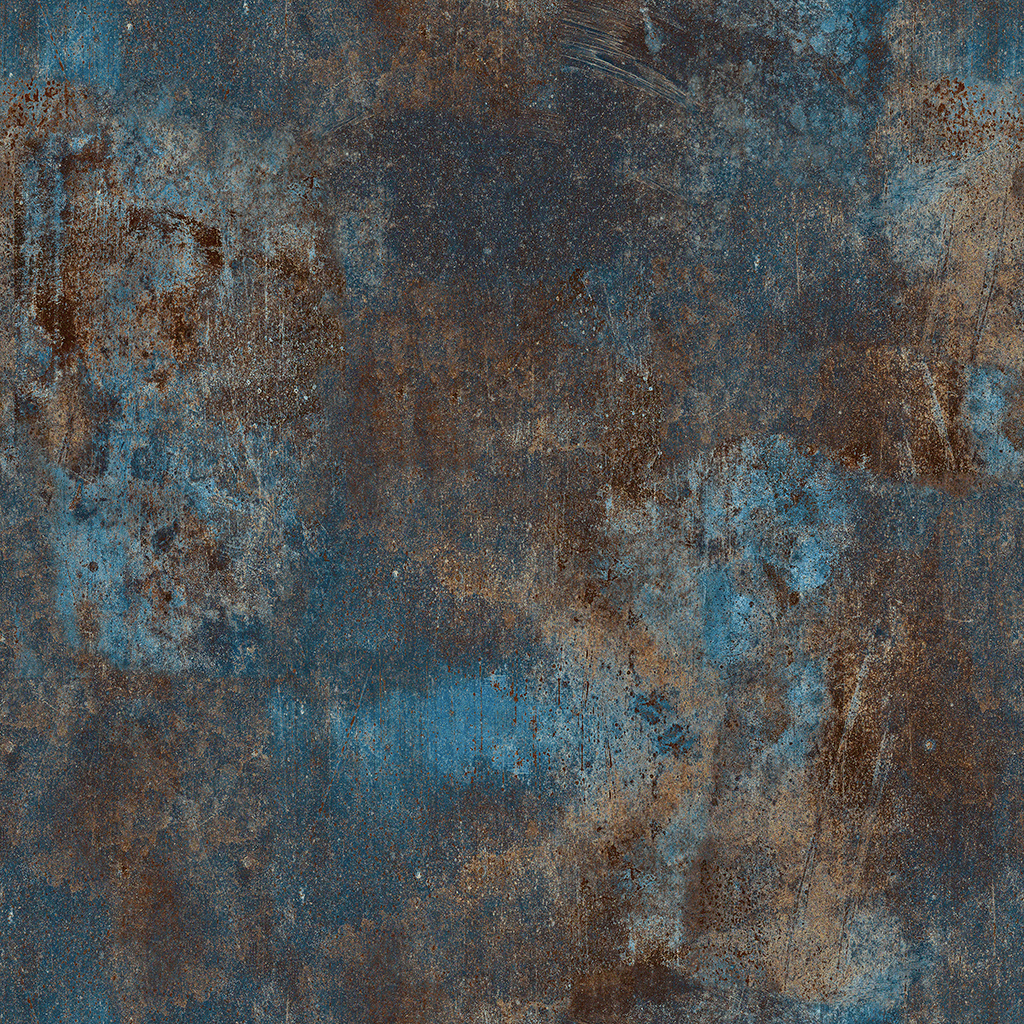
\includegraphics[width=0.42\linewidth]{img/dirty/gt6.png}
% 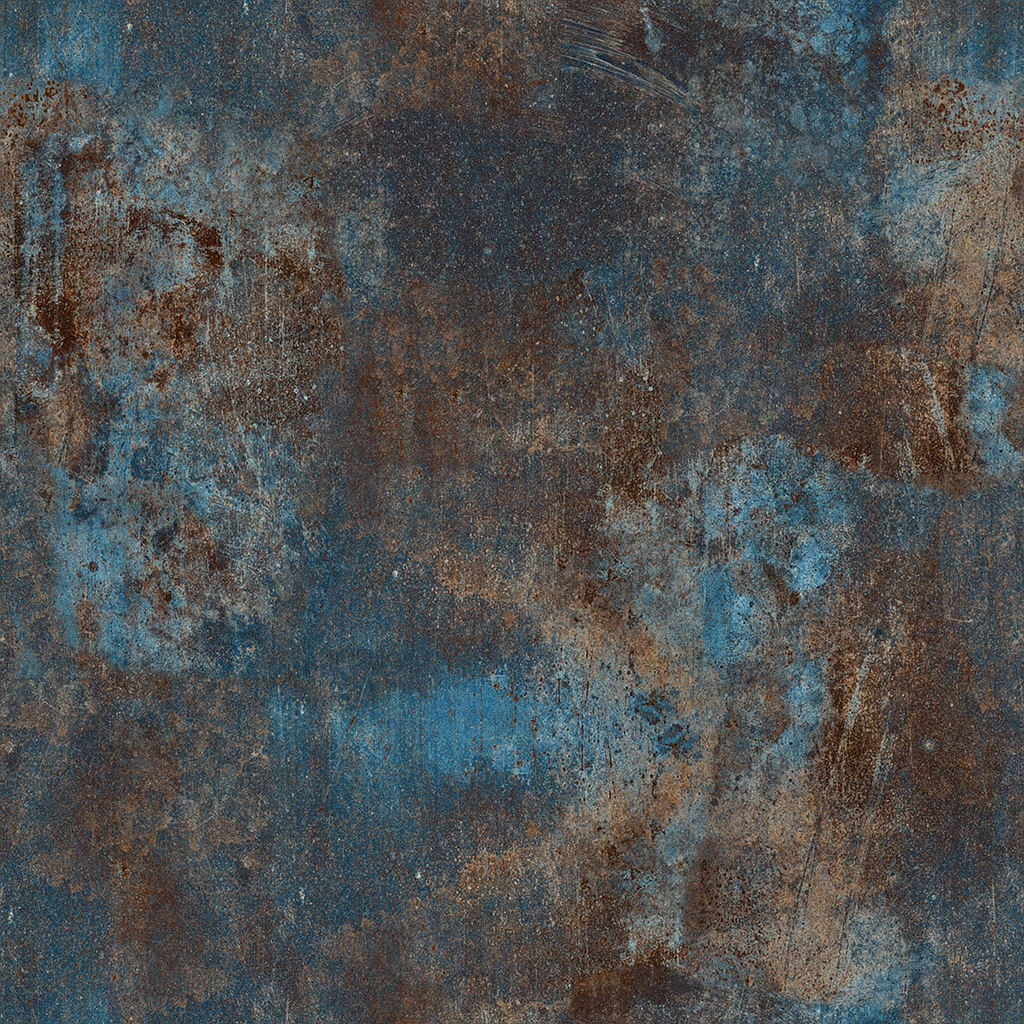
\includegraphics[width=0.42\linewidth]{img/dirty/detail6.png}
% \vspace{-0.4cm}
% \caption{Original image (left); reconstruction of the network (right) 
% }
% \label{f:rec_gt}
% \end{figure}

% To verify the periodicity of our INR model (Secs \ref{s-deep-networks} and \ref{s-mr-networks}), we evaluate the network in a larger domain ($[-2, 2]^2$) than its training domain $[-1, 1]^2$; Figure~\ref{f:mr-periodic} illustrates it for levels of detail 2, 4, and 6.

% \begin{figure}[!h]
% \centering
% \includegraphics[width=0.84\linewidth]{img/dirty/ext.pdf}
% \vspace{-0.4cm}
% \caption{Reconstructed multiresolution levels extrapolation. Top left: level 2; bottom left: level 4; right: level 6.}
% \label{f:mr-periodic}
% \end{figure}

% \subsection{Repeating Patterns in Sample}

% We can also represent a texture with a fundamental period smaller than the sample size. 
% This means that the periodic pattern repeats multiple times within the sample. 
% To address this, we can specify the fundamental period either by prior knowledge or through pre-processing of the image, and train the network using the entire data or only a specific portion of it.

% Figure \ref{f:mask_nomask} showcases a texture sample where the pattern is repeated twice, and its extrapolated reconstructions in the region $[0, 3]^2$. The training considered $[-1, 1]^2$, with a specified period of 1. 
% Figures~\ref{f:mask_nomask} (a) and (c) show the training data, while the network reconstruction is given by (b) and (d), respectively. 
% In (a-b), all coordinates within the region are provided, thus the network learns a periodic representation of the pattern. 
% In (c-d), we employ a mask to exclude a small part while preserving a contiguous region that contains the fundamental period. Again, our method reconstructs the periodic pattern across the entire region. This demonstrates that the over-determined problem does not negatively impact the results. 

% \begin{figure}[!h]
% \centering
% \includegraphics[width=0.24\linewidth]{img/victorian/tile_vitorian.png}
% \includegraphics[width=0.24\linewidth]{img/victorian/extrapolation_nomask.png}
% \includegraphics[width=0.24\linewidth]{img/victorian/train-crab.png}
% \includegraphics[width=0.24\linewidth]{img/victorian/extrapolation-crab.png}
% % \includegraphics[width=0.24\linewidth]{img/victorian/train-face.png}
% % \includegraphics[width=0.24\linewidth]{img/victorian/train-face-mid.png}
% % \includegraphics[width=0.24\linewidth]{img/victorian/extrapolation-face.png}
% % \includegraphics[width=0.24\linewidth]{img/victorian/extrapolation-face-mid.png}
% \vspace{-0.2cm}
% % \includegraphics[width=0.48\linewidth]{img/stochastic_mask.png}
% % \includegraphics[width=0.48\linewidth]{img/extrapolation_randommask.png}
% \centerline{(a)\hfil\hfil(b)\hfil\hfil(c)\hfil\hfil(d)}
% \vspace{-0.4cm}
% \caption{(a) Full training data. (b) Network reconstruction from full data. (c) Masked training data; black pixels were not provided in training. (d) Network reconstruction from masked data.}
% \label{f:mask_nomask}
% \end{figure}

% In the next experiment, a few points have no correspondents visible in any of the periods. This generates an artifact that is noticed across all occurrences of that pattern (Figure \ref{f:artifact}).

% \begin{figure}[!h]
% \centering
% \includegraphics[width=0.27\linewidth]{img/victorian/train-face-mid.png}
% \includegraphics[width=0.27\linewidth]{img/victorian/extrapolation-face-mid.png}
% \includegraphics[width=0.27\linewidth]{img/victorian/artifact.png}
% \vspace{-0.4cm}
% \caption{From left to right: training data, network reconstruction in $[0, 3]^2$, and zoom in one tile to highlight the reconstruction artifact.}
% \label{f:artifact}
% \end{figure}


% Next, we selectively remove points from the training data encouraging a sparse representation of the pattern. We generate the mask by randomly selecting a pixel and subsequently discarding all pixels that correspond to the selected one based on the pattern's period. 
% % These steps are repeated until no additional pixels remain to be sampled. 
% Consequently, the mask encompasses exactly $1/4$ of the total pixels. Figure \ref{f:masked_recontruction} shows the training data, where the black pixels were removed from training, and the learned texture in $[2, 6]^2$. 
% \begin{figure}[!h]
% \centering
% \includegraphics[width=0.4\linewidth]{img/victorian/stochastic_mask.png}
% \includegraphics[width=0.4\linewidth]{img/victorian/extrapolation_randommask.png}
% \vspace{-0.4cm}
% \caption{On the left, the masked input data, where the black pixels were removed from training. On the right, the network reconstruction.~\\
% }
% \label{f:masked_recontruction}
% \end{figure}
% % \vspace{-0.6cm}

% Even in this case, our method captures the underlying periodicity. This provides evidence that we can use the training data at any part of the domain. In other words, we only need a single sample from the class of equivalence defined by the periodicity to reconstruct the image without requiring any additional regularization.

\subsection{Seamless with Poisson Regularization}\label{s:poisson-regularization}

% When obtaining a sample for a material, the inherent irregularity in the sample's pattern poses a challenge in seamlessly stitching it together. Achieving a seamless material is crucial for numerous applications. This section details the application of our methodology to generate seamless results from material patches.

% We train a periodic INR for this task using the loss function of Section~\ref{s-training} which is based on the Poisson equation. In regard to classical Poisson problem solutions, a key observation of our method is the inversion of boundary and interior conditions. 
% We employ masks (the function $\lambda$ in Eq~\ref{e-blending-no-grad}) to delineate the supervision of gradients at the border, while color values are supervised within the interior of the region. Given that our work is situated in the realm of periodic functions, the problem domain is equivalently represented as a torus, thus obviating traditional boundaries.


% While binary masks can produce satisfactory outcomes, they often introduce artifacts at the gradient of the reconstructed network (Figure \ref{f:training_masks}), requiring customized adjusts, per image, of the weights of the loss function components. Consequently, we opted for soft masks computed via a distance function to the center of the mask. 
% In our experiments, we utilized the $L_2$ distance, but any $L_p$ distance can be employed as a parameter for refining the results. 
% \begin{figure}[!h]
% \centering
% 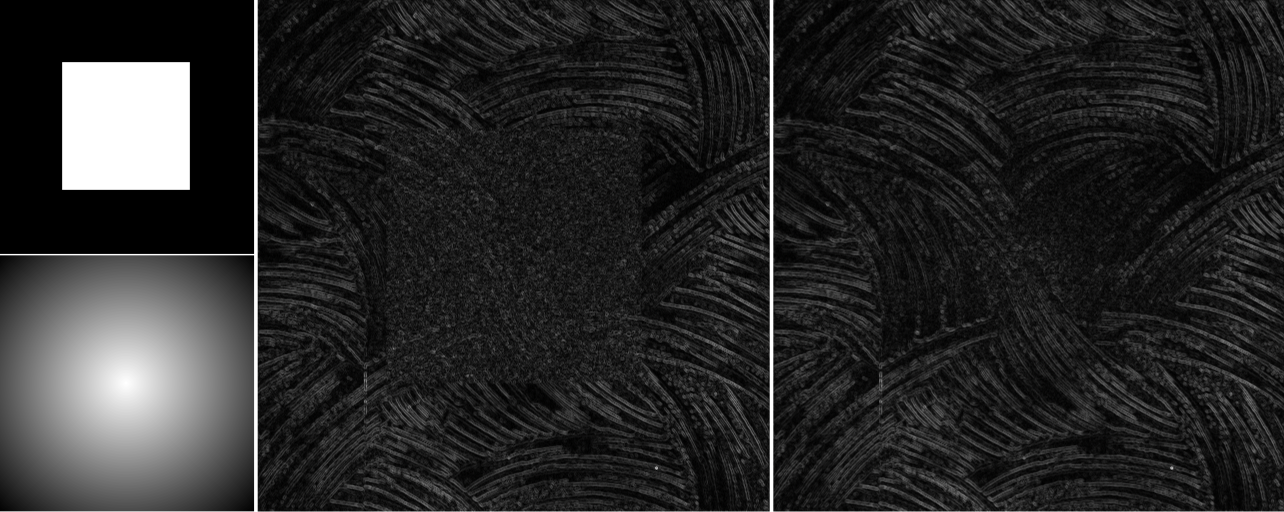
\includegraphics[width=0.90\linewidth]{img/non-tileable/gradients-merged.png}
% % 
\includegraphics[width=0.32\linewidth]{img/non-tileable/hard_mask_d0.png}
% % 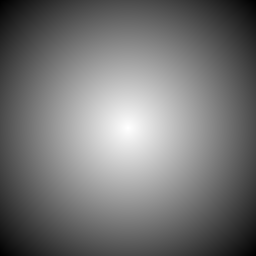
\includegraphics[width=0.32\linewidth]{img/non-tileable/soft_mask_d0.png}

% % 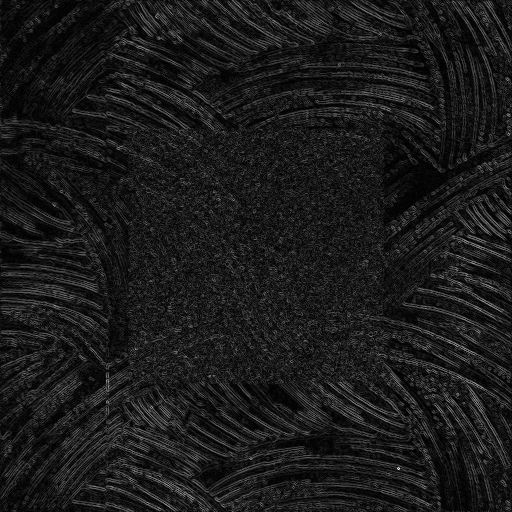
\includegraphics[width=0.32\linewidth]{img/non-tileable/hard_gradient.png}
% % 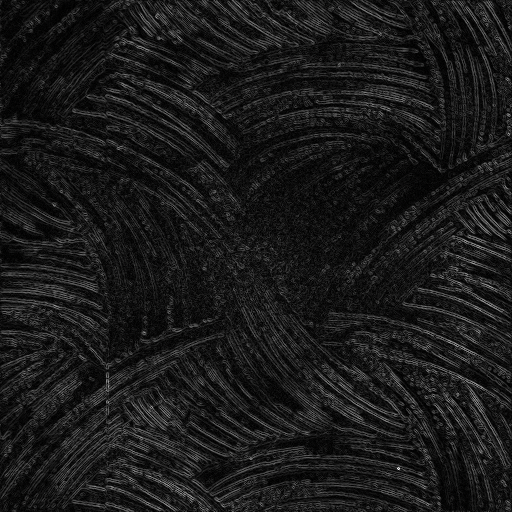
\includegraphics[width=0.32\linewidth]{img/non-tileable/soft_gradient.png}
% \vspace{-0.4cm}
% \caption{Binary mask (top), soft mask (bottom), and the normalized magnitude of the gradients of the trained networks. This is the gradient of the texture in Line 2 of Fig \ref{f:seamless_examples}.}
% \label{f:training_masks}
% \end{figure}

% \vspace{-0.2cm}

% % \begin{figure}[!h]
% % \centering
% % 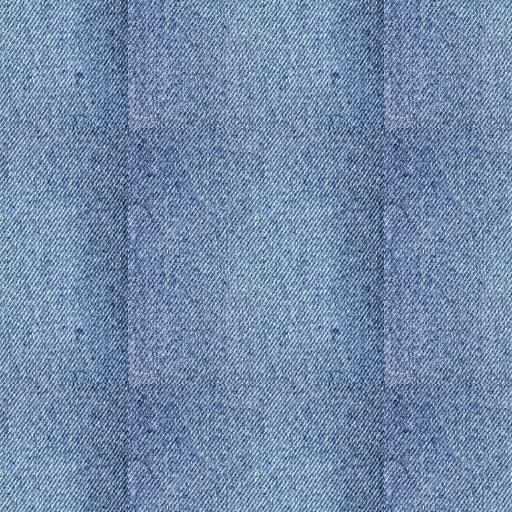
\includegraphics[width=0.40\linewidth]{img/non-tileable/22fabric1.jpg}
% % 
\includegraphics[width=0.40\linewidth]{img/non-tileable/extrapolation_jeans.png}
% % \vspace{-0.2cm}
% % \caption{Seamless reconstruction of jeans fabric}
% % \label{f:extrapolation_jeans}
% % \end{figure}

% % \begin{figure}[!h]
% % \centering
% % 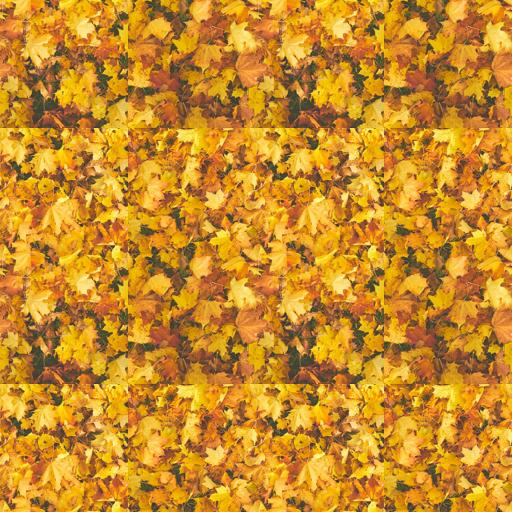
\includegraphics[width=0.38\linewidth]{img/non-tileable/mosaic_leaves.jpg}
% % % 
\includegraphics[width=0.20\linewidth]{img/non-tileable/mask_d1.png}
% % % 
\includegraphics[width=0.20\linewidth]{img/non-tileable/mask_d1.png}
% % 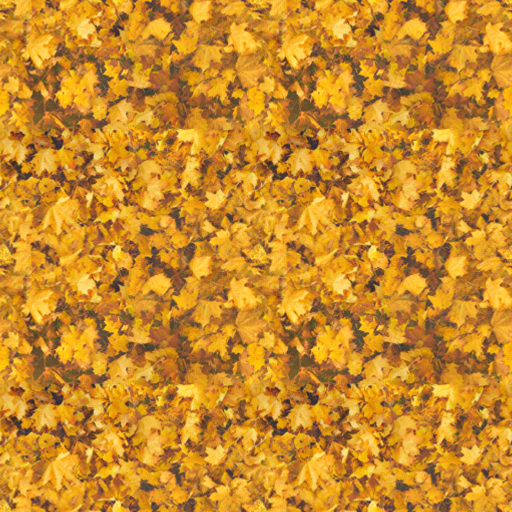
\includegraphics[width=0.38\linewidth]{img/non-tileable/extrapolation-leaves.png}

% % \caption{Wonderful caption}
% % \label{f:seamless_reconstruction}
% % \end{figure}

% Figure~\ref{f:seamless_examples} illustrates several seamless reconstructions (second column) of non-tileable material samples (first column).
% The first line shows an example of a fabric patch containing only fine details.
% The second line gives the case of a pattern featuring medium geometric details. Meanwhile, the third line presents the reconstruction of a pattern characterized by larger details. 
% Note that in all instances, our method adeptly conceals seams through the uniformization of photometric discrepancies. 
% This results in a visually cohesive representation that effectively camouflages the transitions between material patches.
% \begin{figure}[!h]
% \centering
% 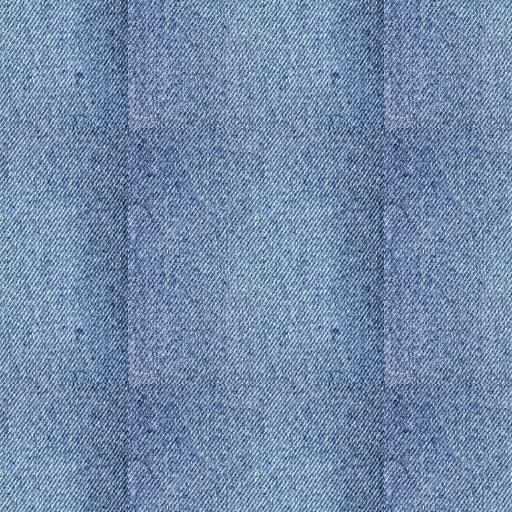
\includegraphics[width=0.43\linewidth]{img/non-tileable/22fabric1.jpg}
% 
\includegraphics[width=0.43\linewidth]{img/non-tileable/extrapolation_jeans.png}
% 
\includegraphics[width=0.43\linewidth]{img/non-tileable/22wall.jpg}
% 
\includegraphics[width=0.43\linewidth]{img/non-tileable/extrapolation_wall.png}
% 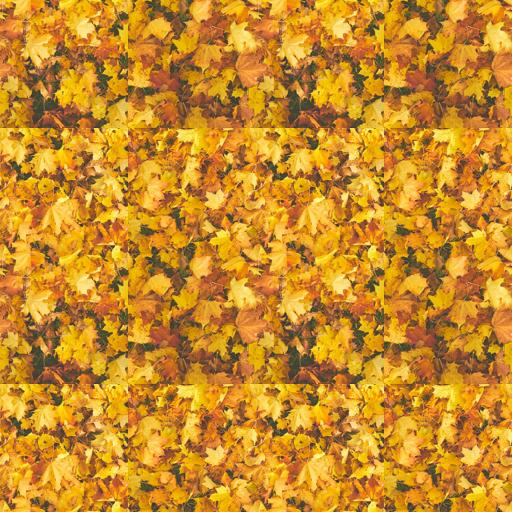
\includegraphics[width=0.43\linewidth]{img/non-tileable/mosaic_leaves.jpg}
% 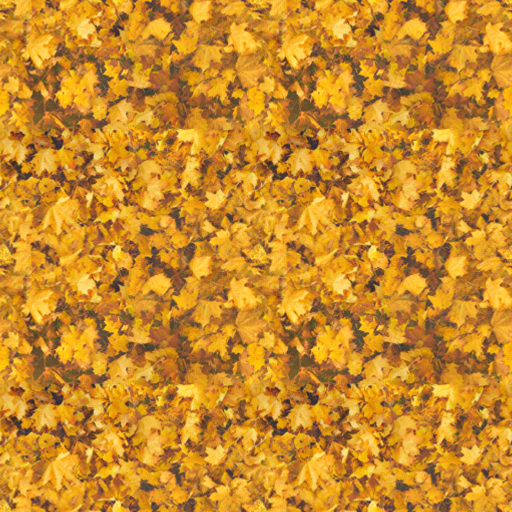
\includegraphics[width=0.43\linewidth]{img/non-tileable/extrapolation-leaves.png}
% \vspace{-0.4cm}
% \caption{Seamless reconstruction of jeans fabric (only fine details), a patch of a wall (medium details). Note that although this texture looks homogeneous it has fine details as can be seen on its gradient in Fig ~\ref{f:training_masks}. Finally, the third line gives the reconstruction of the leaves textures containing big details.
% }
% \label{f:seamless_examples}
% \end{figure}

% % \begin{figure}[!h]
% % \centering
% % 
\includegraphics[width=0.40\linewidth]{img/non-tileable/22wall.jpg}
% % 
\includegraphics[width=0.40\linewidth]{img/non-tileable/extrapolation_wall.png}
% % \vspace{-0.2cm}
% % \caption{Material patch of a wall with intricate details. Note that although this texture looks very homogeneous it has fine details as can be seen on its gradient is on Fig 6.}
% % \label{f:seamless_wall}
% % \end{figure}

% % \vspace{-0.6cm}

% % \begin{figure}[!h]
% % \centering
% % 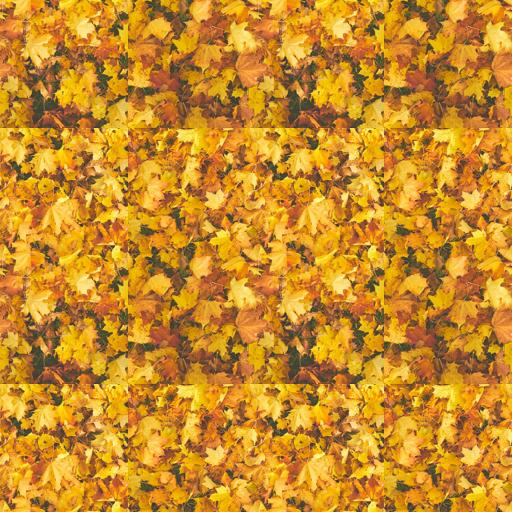
\includegraphics[width=0.40\linewidth]{img/non-tileable/mosaic_leaves.jpg}
% % 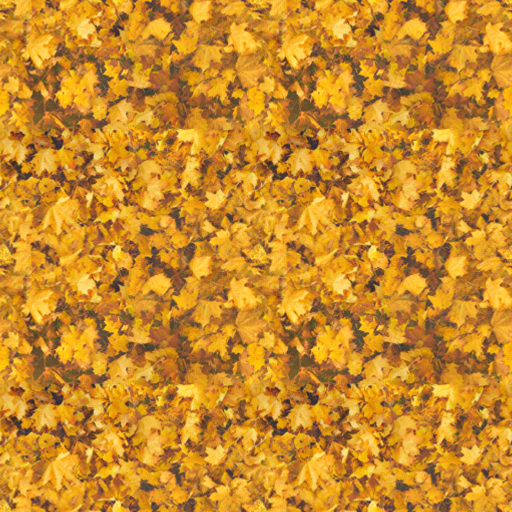
\includegraphics[width=0.40\linewidth]{img/non-tileable/extrapolation-leaves.png}
% % \vspace{-0.2cm}
% % \caption{Texture with big details}
% % \label{f:seamless_leaves}
% % \end{figure}


% % \subsection{Incremental and Compatible Materials}

% % \lnote{red}{
% % Se possivel Fazer o experimento e escrever a seção.
% % dar exemplos de incremental material / compatible material
% % }



% \subsection{Comparisons}

% Here we show that employing periodic activation functions is insufficient for learning periodic images with supervision in a restricted domain. Figure \ref{f:comparison_siren} shows a comparison between image reconstruction/extrapolation using Siren's initialization and our periodic initialization. In this comparison, we use an identical architecture to SIREN: periodic INR with 3 hidden layers, of the form $\R^{256}\to \R^{256}$. The key difference lies in the initialization: we randomly selected 256 pairs of integer frequencies from the range $[0, 30]\times[-30, 30]$, whereas SIREN follows the initialization given in \cite{sitzmann2019siren} with $\omega_0=30$. The images were trained on a $512\times512$ grid within the region $[-1, 1]$ for 500 epochs. The extrapolations are displayed in the interval $[-2, 2]$.


% \begin{figure}[!h]
% \centering
% 
\includegraphics[width=0.43\linewidth]{img/mnet_extrapolation.png}
% 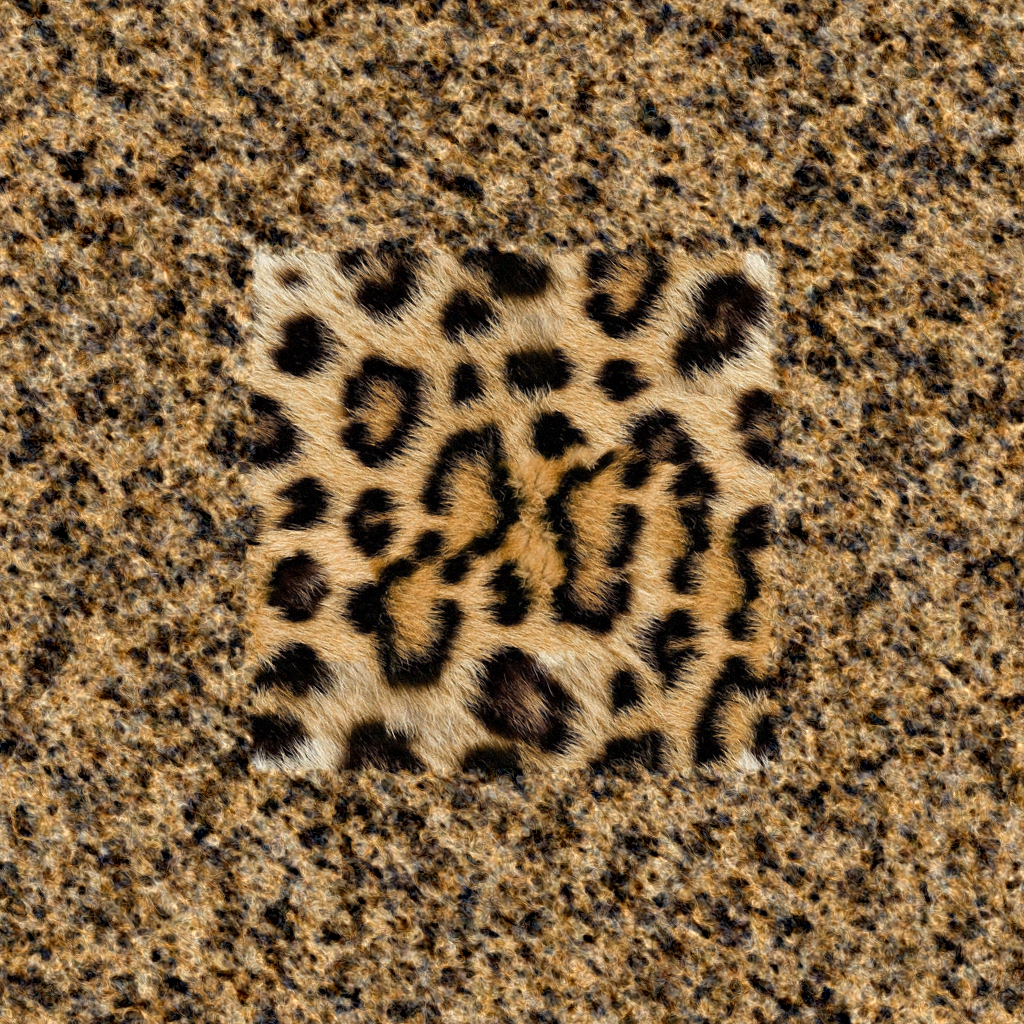
\includegraphics[width=0.43\linewidth]{img/siren_extrapolation.png}
% \vspace{-0.4cm}
% \caption{Comparing our method (left) with Siren (right) on extrapolation.}
% \label{f:comparison_siren}
% \end{figure}

% It is worth noting that, even though the sample image is perfectly tileable, beyond the domain of supervision, the Siren's reconstruction is very noisy, while our approach captures the underlying periodic pattern. 

% We also applied the Poisson regularization, using binary masks, to reconstruct non-tileable patterns in a seamless way using both SIREN and our periodic initialization, see Figure \ref{f:comparison_siren_nontileable}. Again, SIREN's reconstruction displays only noise outside the supervised domain, while our periodic initialization reconstructs a seamless texture.

% \begin{figure}[!h]
% \centering
% 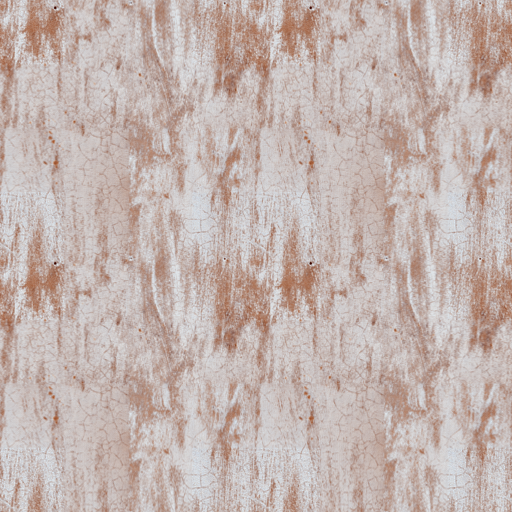
\includegraphics[width=0.47\linewidth]{img/comparisons/mnet_grad_border.png}
% 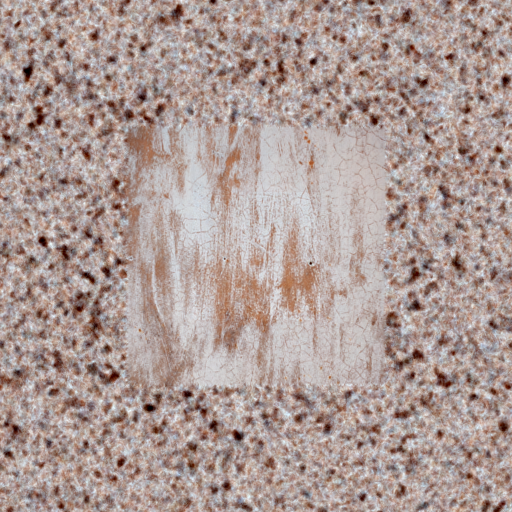
\includegraphics[width=0.47\linewidth]{img/comparisons/siren_grad_border.png}
% \vspace{-0.3cm}
% \caption{Non-tileable patten. Our periodic initialization vs Siren's.}
% \label{f:comparison_siren_nontileable}
% \end{figure}

% % Additionally, we have assessed the effect of our approach on the representation quality of the images and network compactness, regardless of periodicity. To measure this impact, we compute the PSNR for the textures used in Figure~\ref{f:surface_texture_mapping} for sinusoidal models using both Siren's and our periodic initialization. We also compare the reconstruction in multiresolution against \cite{paz2023mr}.
% % % Siren models with 2 hidden layers 256x256, and M-Net models. The M-Net models share the same architecture as ours, as described in section \ref{s-multires-2d}, differing on initialization and training schemes. 
% % Our proposal demonstrated improved representation quality across all examples, as summarized in Table \ref{t:comparison}.

% % \begin{table}[!h]
% % \centering
% % \small
% % \begin{tabular}{|l|r|r|r|}
% % \hline
% % Model & \# Params $(\downarrow)$ & Avg PSNR $(\uparrow)$ \\
% % \hline
% % SIREN 1lvl ~\cite{sitzmann2019siren} & XXX & XXXX dB \\
% % Ours 1lvl & XXX & {\bf XXX} dB  \\
% % M-Net~\cite{paz2022} & 856K & 31.13 dB \\
% % Ours & 856K & {\bf 36.51} dB  \\

% % \hline
% % \end{tabular}
% % % \vspace{-0.1cm}
% % \caption{ Total number of parameters in the models and average PSNR.
% % {\color{red}R3: Table 2 is not conclusive, since SIREN and the proposed approach have nearly 2x difference in parameters.The correct comparison would be one with same number of parameters, like M-Net, and the proposed approach.}
% % }.
% % \label{t:comparison} 
% % \end{table}

% % \vspace{-0.2cm}

% To reconstruct seamless tiles using Poisson equation, \citet{perez2023poisson} suggests to manipulate the pixels intensities at the borders so that left = right and top = bottom, which can be achieved by averaging these values. These intensities should be given as boundary conditions while the gradients should be given at all other positions. In Figure \ref{f:average_border},  we compare this strategy with the one presented in Section \ref{s:poisson-regularization}. Note that our approach gives a more uniform result, better reducing the photometric differences present in the pattern.
% \begin{figure}[!h]
% \centering
% 
\includegraphics[width=0.47\linewidth]{img/comparisons/tile_average-border-inr.png}
% 
\includegraphics[width=0.47\linewidth]{img/comparisons/tile_gradient_border.png}
% \vspace{-0.3cm}
% \caption{Average border (left). Gradient Border (right).}
% \label{f:average_border}
% \end{figure}

% % We also compare our method against traditional Poisson Image Editing (Figure \ref{f:comparison_opencv}).

% % \begin{figure}[!h]
% % \centering
% % \includegraphics[width=0.42\linewidth]{img/comparisons/poisson_opencv.png}
% % \includegraphics[width=0.42\linewidth]{img/comparisons/average_border.png}
% % \vspace{-0.2cm}
% % \caption{Poisson OpenCV vs Average Borders}
% % \label{f:comparison_opencv}
% % \end{figure}

% % * Multiresolution against Bacon
% %     - compare quality of reconstruction
% %     - compare model size

% % \citet{bacon2021} have also used discrete frequencies to initialize Bacon models. Due to the multiplicative characteristic of MFN-based architectures, it was expected that the network would be periodic, and they demonstrated it in an example that we reproduce in Figure \ref{f:comparison_bacon}. However, by eliminating the composition of functions, this kind of network is equivalent to a shallow sinusoidal network where only the amplitude of the frequencies can be learned, while the frequencies themselves are not trained. Consequently, the model needs more parameters to achieve a good reconstruction quality. For instance, a 6 levels Bacon with 256 hidden layers per level for RGB images has a total of 401,991 parameters and achieves a PSNR of 26.51db on the 512x512 image depicted in Figure \ref{f:comparison_bacon}. In contrast, our model reaches 33.0 db in PSNR with 199,985 parameters and 6 levels of multiresolution.


% % \begin{figure}[!h]
% % \centering
% % \includegraphics[width=0.42\linewidth]{img/bacon-ext1024.png}
% % \includegraphics[width=0.42\linewidth]{img/extra_knot.png}
% % \vspace{-0.2cm}
% % \caption{On the left, extrapolation of a Bacon model; on the right, ours.~\\
% % {\color{red}R3: I cannot differentiate between the two images in Figure 10~\\
% % R4: Fig.10: Not sure what this fi gure is implying. The two images look the same.}
% % }
% % \label{f:comparison_bacon}
% % \end{figure}

% % Another drawback of Bacon, specially for multiresolution is that this model builds representations by truncating the image frequency spectra. This approach often introduces ringing artifacts in the image. MR-Net multiresolution more faithfully represents what is expected of successively applying a low-pass filter to an image, and we can leverage it in multiresolution with our initialization, resulting in superior representation quality.

% %     - [ ]  Blending de bordo X Poisson OpenCV
% %     - [ ]  Bordo aberto - falha da Siren? - falha do OpenCV?

% % \vspace{-0.2cm}

% \section{Applications}\label{s-applications}
% % * Anti-aliased surface mapping: 
% % * Anti-aliased solid mapping

% % \tnote{green}{Talvez adicionar um exp que cria uma textura seamless a partir de uma imagem real.}

% \citet{paz2022} have demonstrated MRNet capabilities of encoding mip-mapping and displaying an anti-aliased version of an image, adapted to the required resolution. This section demonstrates practical applications of this property in mapping textures to surfaces.

% \subsection{Surface Texture Mapping}

% We present a simple renderer to show the application of our networks in surface texture mapping (Fig.\ref{f:surface_texture_mapping}). We directly evaluate the network at the $uv$-coordinates of each fragment in a rendering pipeline. 
% First, we map the $uv$-coordinates from the range $[0, 1]$ to  $[-1, 1]$; then, for the torus, we apply a factor of 2 in the $u$ coordinate for a better aspect to the rendering.
% We can also scale the coordinates so that it spans multiple periods of the texture. 

% \pagebreak
% \begin{figure}[!h]
% \centering
% \includegraphics[width=0.24\linewidth]{img/torus/b6.png}
% \includegraphics[width=0.24\linewidth]{img/torus/a6.png}
% \includegraphics[width=0.24\linewidth]{img/torus/d6.png}
% \includegraphics[width=0.24\linewidth]{img/torus/c6.png}
% \includegraphics[width=0.24\linewidth]{img/torus/b6xArnold-cat-map.png}
% \includegraphics[width=0.24\linewidth]{img/torus/a6xfliped.png}
% \includegraphics[width=0.24\linewidth]{img/torus/d6-non-linear.png}
% \includegraphics[width=0.24\linewidth]{img/torus/c6x4.png}
% \vspace{-0.3cm}
% \caption{Neural texture mapping on the torus using its $uv$-coordinates. Line 1 shows four texture examples. Line 2 presents these textures affected by different torus transformations.}
% \label{f:surface_texture_mapping}
% \end{figure}

% % We apply our method to replace an image file in texture mapping using $uv$-coordinates.   To showcase the practical application of our networks in surface texture mapping, we provide a simple renderer (Figure \ref{f:surface_texture_mapping}).

% \vspace{-0.4cm}

% Note that as our network is continuous in space and encodes levels of details, we can evaluate it in any coordinates, and interpolate between levels, akin to Mip-Map \cite{mipmap83}. 
% In this regard, we can perform anti-aliasing similarly to the results in \cite{paz2023mr}.


% % In Figure \ref{f:anti-aliasing}, we reproduce the board in perspective experiment presented in \cite{paz2023mr} using a network trained to make a seamless pattern with 5 multiresolution levels.

% % \begin{figure}[!h]
% % \centering
% % \includegraphics[width=0.42\linewidth]{img/comparisons/naive_sampling.png}
% % \includegraphics[width=0.42\linewidth]{img/comparisons/anti_aliasing.png}
% % \vspace{-0.2cm}
% % \caption{Point sampled texture rendition vs Anti-aliased reconstruction}
% % \label{f:anti-aliasing}
% % \end{figure}

% % {\color{red} R3: I am unsure as to how the multiscale effect is leveraged for mipmapping (as mentioned in line 731). How isthe scale decided at each spatial location?}

% % \lnote{red}{Incluir exemplo de anti-aliasing com MipMap e colocar figura}

% % \lnote{red}{falar tambem sobre deformaçoes no UV usando o iFlow e se possivel colocar exemplo / figura}

% \begin{comment}

% \subsection{Solid Texture Mapping}

% Solid textures offer practical advantages as they eliminate the need for computing $uv$-coordinates on a surface. We trained a solid texture of a marble using Perlin Noise as described in section \ref{s-multires-3d}, and we integrated our representation into the Omniverse platform, which provides a comprehensive rendering pipeline management system. Figure \ref{f:solid_texture_mapping} showcases some of the results achieved using our solid texture mapping approach.

% \begin{figure}[!h]
% \centering
% \includegraphics[width=0.375\linewidth]{img/omniverse/bunny_mrnet.0000.png}
% \includegraphics[width=0.245\linewidth]{img/omniverse/max_plank_mrnet_512_mc400.0099.png}
% \includegraphics[width=0.285\linewidth]{img/omniverse/spot_mrnet.0101.png}
% \caption{Solid Texture Mapping.}
% \label{f:solid_texture_mapping}
% \end{figure}

% To apply the solid texture, we extract meshes from implicit surfaces represented by neural networks and perform the inference of the texture network at the vertices of the mesh. We render the scene using \textit{path tracing}, and we can choose among various materials and shading options to enhance the visual quality of the scene. This demonstrates that this approach can be fully integrated in the  graphics pipeline.

% \end{comment}

% \section{Conclusion and Future Work}

% We presented an unified framework for modeling seamless textures by incorporating Fourier series ideas into neural network architectures. 
% Our approach demonstrates the ability to train the network using partial texture data, making it more compact, and capturing sharper details compared to the ground truth in certain cases.

% While we have made significant progress in understanding the impact of sinusoidal network initialization on representation capacity, there are still paths for future exploration. Although we have constrained the space of frequency choices by selecting integer multiples of a period and partitioning the frequency space, determining the appropriate band limit remains an empirical task. In our current approach, we freeze the weights of the first layer to maintain their constancy throughout training. However, finding a way to make these weights learnable parameters while preserving the desired period is a valuable research direction.

% % Our method has demonstrated effectiveness in 2D/3D texture representations. 

% % \lnote{red}{falar que usamos so' o albedo mas que se aplica naturalmente aos outros canais da definicao de materiais - citar metodos que aprendem os canais a partir de imagens - Substance Image to Materials e Delight - Ref: https://helpx.adobe.com/substance-3d-sampler/filters/tools.html}

% Extending our approach to higher dimensions is a direction for future work. Additionally, exploring the application of our method to represent other graphical objects, such as hypertextures, \citet{hypertexture}, by leveraging the versatility of vector fields in combination with surface representations, holds great potential.

% % \lnote{red}{falar do iFlow - nao exploramos, pois o ponto e' a integracao com o rendering e parametrizacao - talvez citar - "Synthesis of Progressively Variant Textures on Arbitrary Surfaces". ACM Transactions on Graphics, 22(3):295–302, July 2003}

% To fully integrate neural networks as primitives in a graphics pipeline, it is crucial to develop methods for operating and editing them. The functional structure of sinusoidal INRs provides opportunities to explore algebraic structures for network manipulation. 

% % \lnote{red}{naturalmente compacta mas compressao e' trabalho futuro}

% Periodic INRs have high-capacity representation. When restricted to periodic functions domain, they can naturally compress the images, specially in multiresolution. However, investigating compression techniques tailored for sinusoidal networks is essential for achieving compact storage and efficient transmission over computer networks. Exploring the distribution of signal frequencies to inform network initialization is a promising direction in this regard.

% \section{Conclusion and Future Work}


% We demonstrated the effectiveness of our method in 2D/3D texture representations. Furthermore, exploring its extension to higher dimensions to encode time-based animations is a path for future works. 
% Additionally, exploring our method to represent other graphical objects, such as hypertextures \cite{hypertexture}, by leveraging the versatility of vector fields in combination with surface representations, holds great potential.

% To use neural networks as primitives in a graphics pipeline, it is important to develop methods for operating and editing them. 
% The functional structure of sinusoidal networks makes it possible to explore algebraic structures to manipulate such networks.
% Similarly, investigating compression techniques for sinusoidal networks is essential for compact storage and efficient transmission over computer networks. Exploring the signal frequency distribution to inform network initialization is a promising direction in this regard.
% \section{Conclusions}


% In this work we employed \myhl{multiresolution neural networks} to represent periodic textures. By incorporating Fourier series ideas in neural network architectures, we can approximate and model 2D and 3D textures effectively in a unified framework. This approach allowed training the network using only some parts of the texture generator and captures sharper details compared to the ground truth. Integration with other neural graphics frameworks further enhances its potential for texture representation...


% \begin{figure*}[!t]
% \centering
% \includegraphics[width=0.20\linewidth]{img/placeholder.png}
% \includegraphics[width=0.20\linewidth]{img/placeholder.png}
% \includegraphics[width=0.20\linewidth]{img/placeholder.png}
% \includegraphics[width=0.20\linewidth]{img/placeholder.png} \\
% % \vspace{1pt}
% \includegraphics[width=0.20\linewidth]{img/placeholder.png}
% \includegraphics[width=0.20\linewidth]{img/placeholder.png}
% \includegraphics[width=0.20\linewidth]{img/placeholder.png}
% \includegraphics[width=0.20\linewidth]{img/placeholder.png}
% % \vspace{-0.3cm}
% \caption{Reconstructed multiresolution levels extrapolation.}
% \label{f:lod}
% \end{figure*}


% DO NOT INCLUDE ACKNOWLEDGMENTS IN AN ANONYMOUS SUBMISSION TO SIGGRAPH 2019
%\begin{acks}
%
%The authors would like to thank Dr. Maura Turolla of Telecom
%Italia for providing specifications about the application scenario.
%
%The work is supported by the \grantsponsor{GS501100001809}{National
%  Natural Science Foundation of
%  China}{http://dx.doi.org/10.13039/501100001809} under Grant
%No.:~\grantnum{GS501100001809}{61273304\_a}
%and~\grantnum[http://www.nnsf.cn/youngscientists]{GS501100001809}{Young
%  Scientists' Support Program}.
%
%
%\end{acks}

% Bibliography
% \bibliographystyle{ACM-Reference-Format}
% \bibliography{bibliography}


\begin{comment}
% lvelho

\begin{figure*}[!h]
\centering
\includegraphics[width=0.16\textwidth]{img/copper/train1.png}
\includegraphics[width=0.16\textwidth]{img/copper/train2.png}
\includegraphics[width=0.16\textwidth]{img/copper/train3.png}
\includegraphics[width=0.16\textwidth]{img/copper/train4.png}
\includegraphics[width=0.16\textwidth]{img/copper/train5.png}
\includegraphics[width=0.16\textwidth]{img/copper/train6.png}

\includegraphics[width=0.16\textwidth]{img/copper/gfft1.png}
\includegraphics[width=0.16\textwidth]{img/copper/gfft2.png}
\includegraphics[width=0.16\textwidth]{img/copper/gfft3.png}
\includegraphics[width=0.16\textwidth]{img/copper/gfft4.png}
\includegraphics[width=0.16\textwidth]{img/copper/gfft5.png}
\includegraphics[width=0.16\textwidth]{img/copper/gfft6.png}

\includegraphics[width=0.16\textwidth]{img/copper/detail1.png}
\includegraphics[width=0.16\textwidth]{img/copper/detail2.png}
\includegraphics[width=0.16\textwidth]{img/copper/detail3.png}
\includegraphics[width=0.16\textwidth]{img/copper/detail4.png}
\includegraphics[width=0.16\textwidth]{img/copper/detail5.png}
\includegraphics[width=0.16\textwidth]{img/copper/detail6.png}

\includegraphics[width=0.16\textwidth]{img/copper/fft1.png}
\includegraphics[width=0.16\textwidth]{img/copper/fft2.png}
\includegraphics[width=0.16\textwidth]{img/copper/fft3.png}
\includegraphics[width=0.16\textwidth]{img/copper/fft4.png}
\includegraphics[width=0.16\textwidth]{img/copper/fft5.png}
\includegraphics[width=0.16\textwidth]{img/copper/fft6.png}

\includegraphics[width=0.16\textwidth]{img/copper/freq1.png}
\includegraphics[width=0.16\textwidth]{img/copper/freq2.png}
\includegraphics[width=0.16\textwidth]{img/copper/freq3.png}
\includegraphics[width=0.16\textwidth]{img/copper/freq4.png}
\includegraphics[width=0.16\textwidth]{img/copper/freq5.png}
\includegraphics[width=0.16\textwidth]{img/copper/freq6.png}

% \includegraphics[width=0.16\textwidth]{img/copper/ext1.png}
% \includegraphics[width=0.16\textwidth]{img/copper/ext2.png}
% \includegraphics[width=0.16\textwidth]{img/copper/ext3.png}
% \includegraphics[width=0.16\textwidth]{img/copper/ext4.png}
% \includegraphics[width=0.16\textwidth]{img/copper/ext5.png}
% \includegraphics[width=0.16\textwidth]{img/copper/ext6.png}

% \includegraphics[width=0.33\textwidth]{img/copper/ext1.png}
% \includegraphics[width=0.33\textwidth]{img/copper/ext2.png}
% \includegraphics[width=0.33\textwidth]{img/copper/ext3.png}
\includegraphics[width=0.325\textwidth]{img/copper/ext4.png}
\includegraphics[width=0.324\textwidth]{img/copper/ext5.png}
\includegraphics[width=0.325\textwidth]{img/copper/ext6.png}

%
\caption{1st row: train data, the levels of the Gaussian pyramid from coarse to fine. 2nd row: Fast Fourier Transform (FFT) of the expanded pyramid level to the original resolution. 3rd row: all levels of a multiresolution model for the copper texture. 4th row: network inference Fourier spectra. 5th row: the cumulative selected frequencies for initialization of the first layer of each stage. 6th row: extrapolation of the periodic pattern at levels 4, 5, and 6.}
\label{f:ph1}
\end{figure*}

\end{comment}

% \begin{figure*}[!h]
% \centering
% \includegraphics[width=0.4\textwidth]{img/torus/b6.png}
% \includegraphics[width=0.4\textwidth]{img/torus/a6.png}
% \includegraphics[width=0.4\textwidth]{img/torus/a6.png}
% \includegraphics[width=0.4\textwidth]{img/torus/a6.png}
% %
% \caption{.}
% \label{f:ph1}
% \end{figure*}

% Appendix
% \appendix
% \section{Proof of Theorem~\ref{t-periodic}}
% \label{p-theorem}
% In this appendix, 



% \section{Simulator}
% \label{sec:sim}

% If the model checker requests successors of a state which are not
% created yet, the state space uses the simulator to create the
% successors on-the-fly. To create successor states the simulator
% conducts the following steps.
% % enumerate
% \begin{enumerate}
% \item Load state into microcontroller model.
% \item Determine assignments needed for resolving nondeterminism.
% \item For each assignment.
%       \begin{enumerate}
%       \item either call interrupt handler or simulate effect of next instruction, or
%       \item evaluate truth values of atomic propositions.
%       \end{enumerate}
% \item Return resulting states.
% \end{enumerate}
% Figure~\ref{fig:one} shows a typical microcontroller C program that
% controls an automotive power window lift. The program is one of the
% programs used in the case study described in Section~\ref{sec:sim}.
% At first sight, the programs looks like an ANSI~C program. It
% contains function calls, assignments, if clauses, and while loops.
% % Figure
% \begin{figure}
%   \includegraphics{mouse}
%   \caption{Code before preprocessing.}
%   \label{fig:one}
% \end{figure}

% \subsection{Problem Formulation}

% The objective of variable coalescence-based offset assignment is to find
% both the coalescence scheme and the MWPC on the coalesced graph. We start
% with a few definitions and lemmas for variable coalescence.

% % Enunciations
% % \begin{definition}[Coalesced Node (C-Node)]A C-node is a set of
% % live ranges (webs) in the AG or IG that are coalesced. Nodes within the same
% % C-node cannot interfere with each other on the IG. Before any coalescing is
% % done, each live range is a C-node by itself.
% % \end{definition}

% % \begin{definition}[C-AG (Coalesced Access Graph)]The C-AG is the access
% % graph after node coalescence, which is composed of all C-nodes and C-edges.
% % \end{definition}

% % \begin{lemma}
% % The C-MWPC problem is NP-complete.
% % \end{lemma}
% % \begin{proof} C-MWPC can be easily reduced to the MWPC problem assuming a
% % coalescence graph without any edge or a fully connected interference graph.
% % Therefore, each C-node is an uncoalesced live range after value separation
% % and C-PC is equivalent to PC. A fully connected interference graph is made
% % possible when all live ranges interfere with each other. Thus, the C-MWPC
% % problem is NP-complete.
% % \end{proof}

% % \begin{lemma}[Lemma Subhead]The solution to the C-MWPC problem is no
% % worse than the solution to the MWPC.
% % \end{lemma}
% % \begin{proof}
% % Simply, any solution to the MWPC is also a solution to the
% % C-MWPC. But some solutions to C-MWPC may not apply to the MWPC (if any
% % coalescing were made).
% % \end{proof}

% \section{Performance Evaluation}

% During all the experiments, the Geographic Forwarding (GF) by Akyildiz
% et al.~\shortcite{Akyildiz-01} routing protocol is used. GF exploits
% geographic information of nodes and conducts local data-forwarding to
% achieve end-to-end routing. Our simulation is configured according to
% the settings in Table~\ref{tab:one}. Each run lasts for 2 minutes and
% repeated 100 times. For each data value we present in the results, we
% also give its $90\%$ confidence interval.

% % Table
% \begin{table}%
% \caption{Simulation Configuration}
% \label{tab:one}
% \begin{minipage}{\columnwidth}
% \begin{center}
% \begin{tabular}{ll}
%   \toprule
%   TERRAIN\footnote{This is a table footnote. This is a
%     table footnote. This is a table footnote.}   & (200m$\times$200m) Square\\ \midrule
%   Node Number     & 289\\
%   Node Placement  & Uniform\\
%   Application     & Many-to-Many/Gossip CBR Streams\\
%   Payload Size    & 32 bytes\\
%   Routing Layer   & GF\\
%   MAC Layer       & CSMA/MMSN\\
%   Radio Layer     & RADIO-ACCNOISE\\
%   Radio Bandwidth & 250Kbps\\
%   Radio Range     & 20m--45m\\
%   \bottomrule
% \end{tabular}
% \end{center}
% \bigskip\centering
% \footnotesize\emph{Source:} This is a table
%  sourcenote. This is a table sourcenote. This is a table
%  sourcenote.

%  \emph{Note:} This is a table footnote.
% \end{minipage}
% \end{table}%
